\documentclass[12pt,a4paper,notitlepage]{report}
\usepackage[utf8]{inputenc}
\usepackage[polish]{babel}
\usepackage[T1]{fontenc}
\usepackage[top=2cm, bottom=2cm, left=3cm, right=3cm]{geometry}
\usepackage[dvipsnames]{xcolor}
\definecolor{Red}{RGB}{255,36,0}
\usepackage{changepage}
\usepackage{indentfirst}
\usepackage{color}
\usepackage{graphicx}
\definecolor{bluekeywords}{rgb}{0.13,0.13,1}
\definecolor{greencomments}{rgb}{0,0.5,0}
\definecolor{redstrings}{rgb}{0.9,0,0}
\usepackage{listings}
\lstset{language=[Sharp]C,
  showspaces=false,
  showtabs=false,
  breaklines=true,
  showstringspaces=false,
  breakatwhitespace=true,
  escapeinside={(*@}{@*)},
  commentstyle=\color{greencomments},
  keywordstyle=\color{bluekeywords},
  stringstyle=\color{redstrings},
  basicstyle=\ttfamily,
  extendedchars=true
}
\makeatletter
\newcommand{\linia}{\rule{\linewidth}{0.4mm}}
\renewcommand{\maketitle}{\begin{titlepage}
    \vspace*{1cm}
    \begin{center}\small
    Politechnika Wrocławska\\
    Wydział Elektroniki\\
    Urządzenia Peryferyjne 
    \end{center}
    \vspace{4.5cm}
    \noindent\linia
    \begin{center}
      \LARGE \textsc{\@title}
         \end{center}
     \linia
    \vspace{0.5cm}
    \begin{flushright}
    \begin{minipage}{6cm}
    
     \vspace{4cm}
     \textit{\small Termin zajęć:}\\
     \normalsize \textsc{Wtorek TN 7:30} \par
	\vspace{0.3cm}    
    \textit{\small Autorzy:}\\
    \normalsize \textsc{\@author} \par
     \vspace{0.3cm}
        Prowadzący: \\ dr inż. Tomasz Walkowiak

    \end{minipage}
    \vspace{1cm}
     {\small }\\
       
     \end{flushright}
    \vspace*{\stretch{3}}
    \begin{center}
    \@date
    \end{center}
  \end{titlepage}%
}
\makeatother
\author{ Jakub Chmiel  235028 \\ Tomasz Cieślar 235652}
\title{Obsługa joysticka USB z wykorzystaniem DirectInput}
\begin{document}
\maketitle

\newpage
\tableofcontents
\newpage
\renewcommand*\thesection{\arabic{section}}
\section{Cel ćwiczenia}
\begin{enumerate}
\item Korzystając z przykładowej aplikacji stwierdzić obecność joysticka podłączonego do portu USB komputera 
\item Napisać program, odczytujący nazwę zainstalowanego joysticka, wykorzystując w tym celu API DirectInput
\item Napisać program ilustrujący działanie joysticka: stwierdzający naciśnięcie myszy, zmianę położenia drążka (w przestrzeni 2D) oraz suwaka.
\item Napisać program zastępujący działanie myszy. Program ma umożliwiać sterowanie kursorem za pomocą joysticka oraz obsługę przycisków fire jako kliknięć myszy.
\item Napisać program realizujący prosty edytor graficzny - rysowanie przy pomocy Joysticka
\end{enumerate}

\section{Wstęp}
DirectInput jest to biblioteka obsługująca urządzenia wejściowe tj. klawiatura, mysz czy joystick, będąca częścią DirectX firmy Microsoft. Zawiera w sobie funkcje odczytujące dane z tych urządzeń w różny sposób (bezpośredni lub buforowany). Ma też możliwość przyporządkowania określonych akcji do konkretnych przycisków (Action Mapping). DirectInput nie przyniesie żadnych dodatkowych korzyści aplikacjom, które używają klawiatury do wprowadzania tekstu i myszy do nawigacji. API jest przeznaczone głównie do tworzenia gier komputerowych, symulacji i wszystkich innych interaktywnych aplikacji dla Windows.
\section{Założenia projektowe}
\begin{itemize}
\item Program był pisany w języku C\texttt{\#}.
\item Na komputerze, na którym uruchamiany był program zainstalowano system operacyjny Windows 10 w wersji 64-bitowej.
\end{itemize}

\section{Wykorzystane narzędzia}
\begin{itemize}
\item Windows Forms - API do implementacji interfejsu graficznego dla platformy .NET.
\item SlimDX - API dla programowania z użyciem DirectX na platformie .NET.
\end{itemize}
\begin{adjustwidth}{0pt}{-50pt}
\section{Implementacja programu}
\subsection{Interfejs aplikacji}
\begin{center}
\noindent 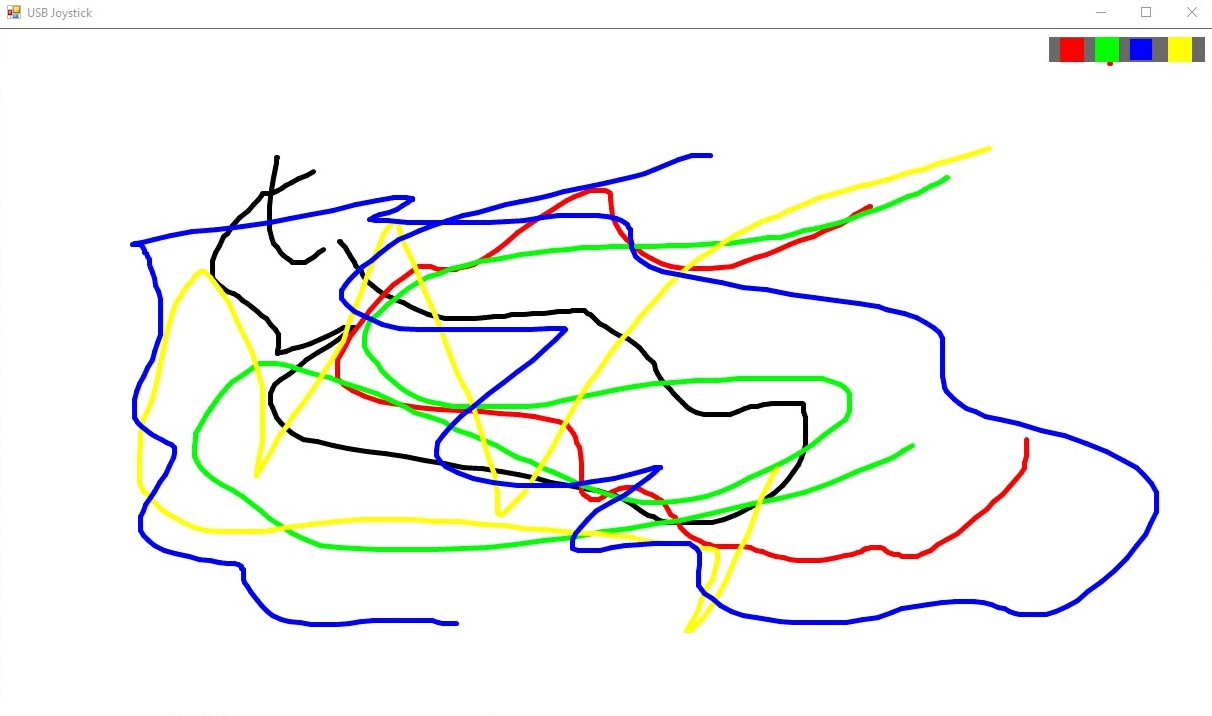
\includegraphics[scale=0.45]{okno}
\\
\begin{normalsize}
\textit{Rysunek 1. Interfejs aplikacji}
\end{normalsize}
\end{center}
\subsection{Kod źródłowy}
\begin{lstlisting}
using [...]

namespace USB
{
    public partial class Form1 : Form
    {
        Graphics g;
        private int x = -1;
        private int y = -1;
        private bool moving = false;
        private Pen pen;
        private Color currentColor = Color.Black;
        private Color previousColor = Color.Black;
        private Color currColor = Color.Black;
        private bool prev = false;
        
        public Form1()
        {
            InitializeComponent();
            GetSticks();
            Sticks = GetSticks();
            timer1.Enabled = true;
            //Przygotowanie panelu do rysowania
            g = panel1.CreateGraphics();
            g.SmoothingMode = System.Drawing.Drawing2D.SmoothingMode. AntiAlias;
            pen = new Pen(Color.Black, 5);
            pen.StartCap = pen.EndCap = System.Drawing.Drawing2D.LineCap.Round;
        }
		
		//
        DirectInput Input = new DirectInput();
        SlimDX.DirectInput.Joystick stick;
        Joystick[] Sticks;

        bool mouseClicked = false;

        int yValue = 0;
        int xValue = 0;
        int zValue = 0;

        [DllImport("user32.dll", CharSet = CharSet.Auto)]
        public static extern void mouse_event(uint flag, uint _x, uint _y, uint btn, uint exInfo);
        private const int MOUSEEVENT_LEFTDOWN = 0x02;
        private const int MOUSEEVENT_LEFTUP = 0x04;
        
        public Joystick[] GetSticks()
        {
        	//Lista podlaczonych urzadzen typu joystick
            List<SlimDX.DirectInput.Joystick> sticks = new List<SlimDX.DirectInput.Joystick>();
            foreach (DeviceInstance device in Input.GetDevices(DeviceClass.GameController, DeviceEnumerationFlags.AttachedOnly))
            {
                try
                {
                	//Pobranie informacji o urzadzeniu
                    stick = new SlimDX.DirectInput.Joystick(Input, device.InstanceGuid);
                    stick.Acquire();

                    foreach(DeviceObjectInstance deviceObject in stick.GetObjects())
                    {
                        if((deviceObject.ObjectType & ObjectDeviceType.Axis) != 0)
                        {
                            stick.GetObjectPropertiesById ((int)deviceObject.ObjectType). SetRange(-100, 100);
                        }
                    }
                    sticks.Add(stick);
                }
                catch (DirectInputException)
                {
                    
                }
            }
            return sticks.ToArray();
        }

        void stickHandle(Joystick stick, int id)
        {
        	//Obsluga joysticka
            JoystickState state = new JoystickState();
            state = stick.GetCurrentState();
           
            //Wychylenia osi X, Y, Z
            yValue = state.Y;
            xValue = state.X;
            zValue = state.Z;
            pen.Width = (float)((zValue + 101) * 0.2);
            MouseMove(xValue, yValue);

			//Pobranie stanow przyciskow
            bool[] buttons = state.GetButtons();

            if(id == 0)
            {
                if (buttons[1])
                {
                	//Czyszczenie panelu
                    panel1.BackColor = Color.White;
                    panel1.Refresh();
                }
                if (buttons[2])
                {
                	//Przelaczanie miedzy ostatnimi dwoma kolorami
                    if (prev)
                    {
                        pen.Color = currentColor;
                        prev = false;
                    }
                    else
                    {
                        pen.Color = previousColor;
                        prev = true;
                    }

                    currColor = pen.Color;
                }
                if (buttons[0])
                {
                	//Rysowanie (wcisniecie lewego przycisku myszy)
                    if (mouseClicked == false)
                    {
                        mouse_event(MOUSEEVENT_LEFTDOWN, 0, 0, 0, 0);
                        mouseClicked = true;
                    }
                }
                else
                {
                	//Zwolnienie LPM
                    if(mouseClicked == true)
                    {
                        mouse_event(MOUSEEVENT_LEFTUP, 0, 0, 0, 0);
                        mouseClicked = false;
                    }
                }
            }
        }

        public void MouseMove (int posx, int posy)
        {
        	//Poruszanie kursorem
            Cursor.Position = new Point(Cursor.Position.X + posx/3, Cursor.Position.Y + posy/3);
            Cursor.Clip = new Rectangle(this.Location, this.Size);

        }

        private void timer1_Tick(object sender, EventArgs e)
        {
        	//Obsluga timera, ktory wywoluje metode zbierajaca informacje o aktualnym stanie joysticka
            for (int i = 0; i < Sticks.Length; i++)
            {
                stickHandle(Sticks[i], i);
            }
        }

        private void Form1_Load(object sender, EventArgs e)
        {
            Joystick[] joystick = GetSticks();
        }

        private void pictureBox1_Click(object sender, EventArgs e)
        {
        	//Przelaczanie kolorow
            pictureBox1.BorderStyle = BorderStyle.None;
            pictureBox2.BorderStyle = BorderStyle.None;
            pictureBox3.BorderStyle = BorderStyle.None;
            pictureBox4.BorderStyle = BorderStyle.None;
            
            PictureBox p = (PictureBox) sender;

            pen.Color = p.BackColor;
            previousColor = currColor;
            currentColor = p.BackColor;

            if (p.BorderStyle == BorderStyle.FixedSingle)
            {
                p.BorderStyle = BorderStyle.None;
                pen.Color = Color.Black;
            }
            else
            {
                p.BorderStyle = BorderStyle.FixedSingle;
            }
        }

        private void panel1_MouseUp(object sender, MouseEventArgs e)
        {
        	//Zwolnienie LPM - koniec rysowania
            moving = false;
            x = -1;
            y = -1;
            panel1.Cursor = Cursors.Default;
        }

        private void panel1_MouseDown(object sender, MouseEventArgs e)
        {
        	//Wcisniecie LPM - rozpoczecie rysowania
            moving = true;
            x = e.X;
            y = e.Y;
            g.DrawLine(pen, new Point(x, y), new Point(x + 1, y));
            panel1.Cursor = Cursors.Cross;
        }

        private void panel1_MouseMove(object sender, MouseEventArgs e)
        {
        	//Poruszanie mysza - rysowanie linii
            if (moving && x != -1 && y != -1)
            {
                g.DrawLine(pen, new Point(x, y), e.Location);
                x = e.X;
                y = e.Y;
            }
        }
    }
}

\end{lstlisting}

\end{adjustwidth}
\section{Wnioski}
Udało nam się wykonać zadanie w całości. Joystick przejmował operację kursora myszki i umożliwiał rysowanie na panelu w oknie aplikacji. API SlimDX znacząco ułatwiło obsługę urządzenia.
\section{Bibliografia}
\begin{itemize}
\item DirectInput:
\\
$https://en.wikipedia.org/wiki/DirectInput$
\item Dokumentacja SlimDX:
\\
$https://slimdx.org/docs/$
\end{itemize}

\end{document}